\section{Extensible Backend}
\subsection{Chat Bot}
\subsubsection{Process}
\begin{enumerate}
    \item{The user sends a query to the chat bot via the web interface.}
    \item{The chat bot sends the query to Dialogflow to extract the keywords and intents.}
    \item{It will then search the database to find candidate responses.}
    \item{A score is calculated for each candidate based on its theta value and salience.}
    \item{The candidate with the highest score is considered the best answer.}
    \item{When deciding on a response, the chat bot also considers whether or not the user's query is a question.}
    \item{The final chosen answer is returned to the user via the web interface.}
\end{enumerate}

\subsubsection{Example Usage}
The user accesses the chat interface and sends a greeting message. This is parsed and detected as a "Default Welcome Intent", and the bot responds accordingly.

\begin{center}
    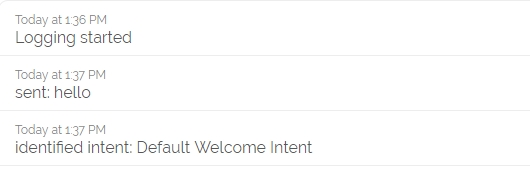
\includegraphics[width=7cm]{log1.png}
\end{center}

The user then asks "What is fork?" This query is also processed and the intent is identified as corresponding to the course content. The chat bot queries the database and chooses from the answers with the highest score. The answer with the highest score is displayed at the top in the debug log shown below.

\begin{center}
    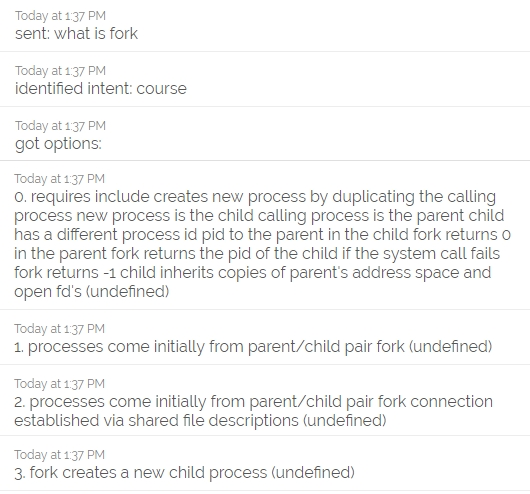
\includegraphics[width=7cm]{log2.png}
\end{center}

\subsubsection{Technical Details}
The chat bot is retrieval-based and functions on two layers. The initial layer is the Dialogflow component. It handles the natural language processing of the user query and extracts keywords, as well as dealing with responses for non-relevant questions. Dialogflow was chosen as it is a known, reliable module and has core NLP features such as small talk, which help our bot appear more human. It also has an API for communication with our backend, which suited our needs perfectly.

The second layer of our chat bot is custom query fulfillment, which finds relevant data to return to the user to answer their question. The database is searched for candidates that contain the keywords extracted by dialogflow. A relevance score is then calculated for each data candidate, based on the theta and salience values of tags matching the user's keywords, and the most relevant data is sent to the user.

Our system uses an initial data set which is approved content by the course lecturer, and contains answers relevant to students of that specific course. The chatbot uses feedback from users to increase or decrease the theta values of each data item, so that it can learn the correct responses over time. Our system has adjustable training sensitivity to speed up the initial training process, and it is able to retrieve some useful data points without any prior training.

\subsection{Internal APIs}
\subsubsection{Process}
\begin{enumerate}
    \item{The backend API runs in its own instance, separate from the frontend.}
    \item{The user makes a request via the interface on the frontend.}
    \item{The frontend sends an \code{HTTP} request to the API with the details of the user's request.}
    \item{The API receives the request and routes it appropriately.}
    \item{The corresponding function is called and handles the user's request.}
    \item{An \code{HTTP} response is sent back to the frontend based on the behaviour of the function.}
    \item{The frontend displays an appropriate response to the user based on the response it receives.}
\end{enumerate}

\subsubsection{Usage}
The internal API is accessed when a user wants to register. When accessing the homepage, the user will see a registration form. Using this, they can choose a name and confirm it by pressing the button.

\begin{center}
    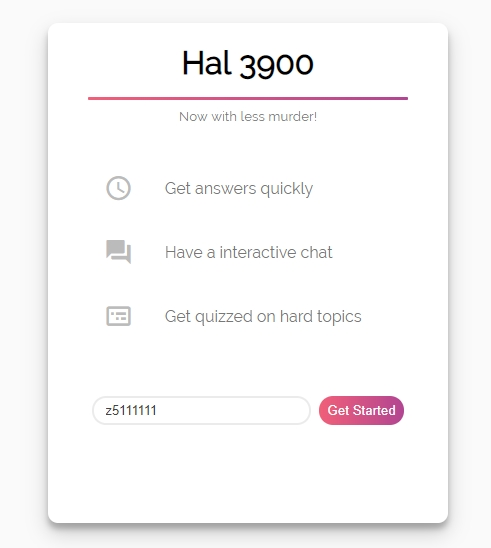
\includegraphics[width=7cm]{register.jpg}
\end{center}

The \code{Get Started} button sends an \code{HTTP POST} request to the internal API at a specific URL. The backend router associates this with the function to register or log in a user. The function runs, and checks if the user already exists. If they do, their previous session will be loaded. Otherwise, a new session will be created for the user. The API then sends an \code{HTTP} response back to the frontend and the user can proceed to use the system.

\begin{center}
    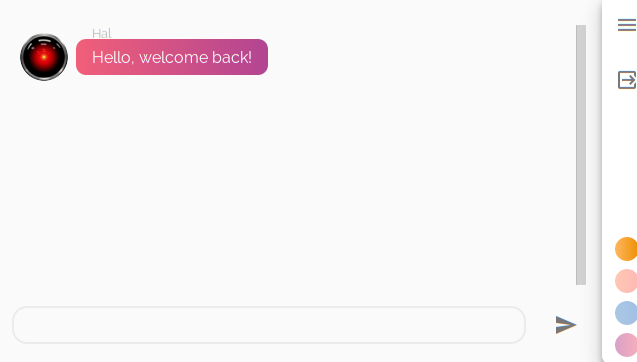
\includegraphics[width=\textwidth]{welcome.png}
\end{center}

\subsubsection{Technical Details}
The backend is primarily constructed using \code{Node.js} in \code{TypeScript}. It was chosen due to its high amount of usage in the industry and abundance of packages and documentation that could be taken advantage of. One of the main advantages of using \code{Node.js} over something like \code{Django} for example, is the availability of an easy-to-use web socket implementation. This allowed us to easily create a real-time chat system, which is part of our core functionality.

\code{Express.js} and \code{express-session} were used to handle routing and user sessions, respectively. Considering there was already a reliable implementation of these core but basic features, we did not see a need to create our own. Similarly, \code{express-ws} was used to deal with the web socket functionality that we needed.

\code{TypeScript} was chosen mainly for development purposes. It helped to ensure our code was robust and error free by enforcing data types to avoid common \code{JavaScript} errors.

\newpage
